\chapter{Concepto de anomalía}
\label{chapter:anomalia}

\section{Contextualización}

Ya hemos discutido previamente una idea intuitiva del concepto de anomalía. Un dato decimos que es anómalo cuando se distancia del resto de los datos lo suficiente como para no tener características comunes con el resto.

Este hecho puede ser por distintos motivos. Puede que la anomalía venga del hecho de que se está produciendo un evento en nuestros experimentos que no sea nada frecuente. Por ejemplo podemos estar midiendo datos meteorológicos y que en un momento dado se den una serie de fenómenos que no sea frecuente ver juntos, o incluso que no se hayan visto nunca ocurrir simultáneamente. Otra forma de tener una anomalía en nuestro conjunto de datos pudiera ser errores de medición. Por ejemplo si seguimos con este símil de los datos meteorológicos imaginemos que nuestra estación dispone de un termómetro. Este sensor se ha roto y empieza a marcar datos superiores a 100 $C^\circ$, claramente son datos muy desviados de las temperaturas normales con lo que no tendrían relación con el resto y presentaría una desviación muy importante con respecto al resto de los datos.

\section{Criterios}

Esta idea intuitiva que estamos dando de anomalía no refleja todos los posibles escenarios. Los ejemplos que estamos dando suponen una desviación muy grande de los datos normales, tanto que no se pueden comparar con el resto porque difieren mucho numéricamente. Vamos a plantear un escenario para dar una mejor forma al concepto de anomalía. Pensemos en una serie de datos muy agrupados en dos clústers por ejemplo:

\begin{figure}[H]
	\centering
	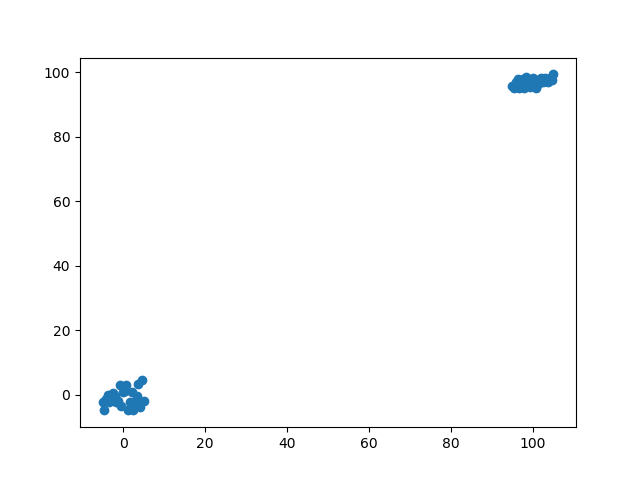
\includegraphics[scale=0.5]{imagenes/clusters}
	\label{clusters}
	\caption{Clusters alejados}
\end{figure}

Como podemos comprobar que tenemos dos clústers no sólo alejados entre sí, si no con los elementos muy concentrados para poner un caso extremo. Ahora no vamos a proponer un valor que se aleje de los dos clústers, si no uno que esté a medio camino entre los dos:

\begin{figure}[H]
	\centering
	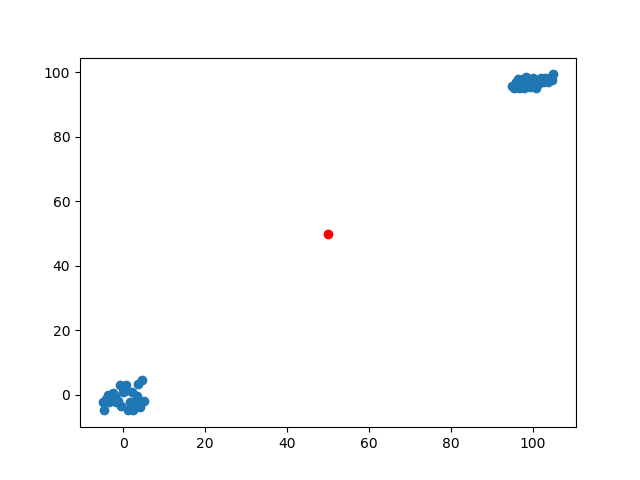
\includegraphics[scale=0.5]{imagenes/outlier_cluster}
	\label{outlier_clusters}
	\caption{Clusters alejados con una anomalía en rojo}
\end{figure}

Si los datos del clúster de abajo a la izquierda fueran datos de temperatura con valores entorno a 0 y los de arriba a la derecha fueran de datos de temperatura entorno a 100 grados nuestro datos anómalo tendría una temperatura de unos 50 grados. Esta temperatura no se aleja radicalmente de los valores normales, es decir, no son -1000 grados ni 1000 grados. Aún así estamos describiendo una situación anómala.

No podemos dar una definición formal o que podamos decir que abarca todos los casos para definir lo que es una anomalía, aún así vamos a intentar dar dos puntos de vista: uno basado en distancias y otro en probabilidades.

El criterio más usado en la definición o detección de anomalías es el llamado ``Tukey's Fences''. Para introducirlo vamos a ver su definición en una única dimensión para luego extender el concepto. Pensemos en un conjunto de datos 1-D. Sobre sus valores podemos calcular los cuartiles $Q_1 , Q_2 $ y $Q_3$. Un valor anómalo es aquel que no cae dentro del intervalo $[Q_1 - k(Q_3 - Q_1), Q_3 + k(Q_3 - Q_1)]$ donde $k$ es una constante. El valor propuesto para $k$ por Tukey fue de $k=1.5$ aunque algunos autores más restrictivos proponen $k=3$.

Este criterio puede ser extendido al caso de mayor dimensionalidad si realizamos este mismo test sobre todos los valores de todas las características y comprobar si alguno o todos se salen del rango en función de cómo de restrictivo queremos que sea el criterio.

Esta extensión es muy vaga, por lo que se propone un criterio un poco más fijado. Imaginemos los datos agrupados por clústers, entonces podemos fijar un centroide de dicho cluster. Sobre cada cluster podemos medir cuál es la mayor distancia intercluster de los datos al centroide. Podemos extender el criterio de Tukey diciendo que un dato anómalo es aquel que se distancia más de $1.5$ veces de la mayor distancia intercluster al centroide.

Esta generalización ya si abarca el ejemplo que hemos propuesto. Al estar muy apiñados los datos entorno al centroide la mayor distancia intercluster es muy pequeña, de hecho en el ejemplo construido es menor que 5. Por tanto el dato $(50,50)$ está alejado más de $1.5 \cdot 5 = 7.5$ unidades del centroide y por tanto lo podemos considerar una anomalía.